%compile with pdflatex on papeeria

\documentclass[a4paper,12pt]{article}
\usepackage{fancyhdr}
\usepackage{fancyheadings}
\usepackage[ngerman,german]{babel}
\usepackage{german}
\usepackage[utf8]{inputenc}
%\usepackage[latin1]{inputenc}
\usepackage[active]{srcltx}
%\usepackage{algorithm}
%\usepackage[noend]{algorithmic}
\usepackage{amsmath}
\usepackage{amssymb}
\usepackage{amsthm}
\usepackage{bbm}
\usepackage{enumerate}
\usepackage{graphicx}
\usepackage{ifthen}
\usepackage{listings}
\usepackage{enumitem}
%\usepackage{struktex}
\usepackage{hyperref}
\usepackage{tikz}
\usepackage{float}
\usepackage{subcaption}
\usepackage{array}
\captionsetup{compatibility=false}
\captionsetup[subfigure]{labelformat=empty}

\usepackage{pgfplots}
\pgfplotsset{compat=1.15}
\usepackage{mathrsfs}
\usetikzlibrary{arrows}

\definecolor{ccqqqq}{rgb}{0.8,0,0}
\definecolor{kolorwykresu}{rgb}{0.07,0.04,0.56}

\pagenumbering{gobble}

\usepackage{tabularray}
\usepackage{multirow}
\usepackage{booktabs,tabularx}
\renewcommand\tabularxcolumn[1]{m{#1}}% for vertical centering text in X column

\newcolumntype{L}[1]{>{\raggedright\let\newline\\\arraybackslash\hspace{0pt}}m{#1}}
\newcolumntype{C}[1]{>{\centering\let\newline\\\arraybackslash\hspace{0pt}}m{#1}}
\newcolumntype{R}[1]{>{\raggedleft\let\newline\\\arraybackslash\hspace{0pt}}m{#1}}

\newcolumntype{Y}{>{\centering\arraybackslash}X}

%%%%%%%%%%%%%%%%%%%%%%%%%%%%%%%%%%%%%%%%%%%%%%%%%%%%%%
%%%%%%%%%%%%%% EDIT THIS PART %%%%%%%%%%%%%%%%%%%%%%%%
%%%%%%%%%%%%%%%%%%%%%%%%%%%%%%%%%%%%%%%%%%%%%%%%%%%%%%
\newcommand{\Fach}{2. Klausur aus der Mathematik (A)}
\newcommand{\Name}{}
\newcommand{\datum}{}
\newcommand{\Matrikelnummer}{}
\newcommand{\Semester}{Q11/2}
\newcommand{\Uebungsblatt}{} %  <-- UPDATE ME
%%%%%%%%%%%%%%%%%%%%%%%%%%%%%%%%%%%%%%%%%%%%%%%%%%%%%%
%%%%%%%%%%%%%%%%%%%%%%%%%%%%%%%%%%%%%%%%%%%%%%%%%%%%%%

\setlength{\parindent}{0em}
\topmargin -1.0cm
\oddsidemargin 0cm
\evensidemargin 0cm
\setlength{\textheight}{9.2in}
\setlength{\textwidth}{6.0in}

%%%%%%%%%%%%%%%
%% Aufgaben-COMMAND
\newcommand{\Aufgabe}[1]{
  {
  \vspace*{0.5cm}
  \textsf{\textbf{Aufgabe #1}}
  \vspace*{0.2cm}
  
  }
}
%%%%%%%%%%%%%%
\hypersetup{
    pdftitle={\Fach{}: Übungsblatt \Uebungsblatt{}},
    pdfauthor={\Name},
    pdfborder={0 0 0}
}

\lstset{ %
language=java,
basicstyle=\footnotesize\tt,
showtabs=false,
tabsize=2,
captionpos=b,
breaklines=true,
extendedchars=true,
showstringspaces=false,
flexiblecolumns=true,
}

\title{Übungsblatt \Uebungsblatt{}}
\author{\Name{}}

\begin{document}

\fancyhead{}
\fancyhead[C]{
\includegraphics[height=2.5cm]{lukasLogo.png}
\vspace{2cm}
}

\thispagestyle{fancy}

\lhead{
%\vspace{1cm}
  \sf \LARGE \Fach{} %\small \Name{} - \Matrikelnummer{}
}
\rhead{\sf \Semester{}   \datum{}}

\vspace*{0.2cm}

\vspace{4cm}
Alle Lösungen müssen mit Nebenrechnungen und Begründungen nachvollziehbar sein!

%\rhead{\sf \Semester{} }
\vspace*{0.2cm}

%\begin{center}
%%\LARGE \sf \textbf{Übungsblatt \Uebungsblatt{}}
%\end{center}
%\vspace*{0.2cm}

%%%%%%%%%%%%%%%%%%%%%%%%%%%%%%%%%%%%%%%%%%%%%%%%%%%%%%
%% Insert your solutions here %%%%%%%%%%%%%%%%%%%%%%%%
%%%%%%%%%%%%%%%%%%%%%%%%%%%%%%%%%%%%%%%%%%%%%%%%%%%%%%

\vspace{1cm}
  Name: \underline{\hspace{7cm}}
  \hfill
  Datum: \underline{\hspace{4cm}}

\vspace{0.8cm}

Zeit: 90 Minuten
%\vspace{0,5cm}Die Rechenwege müssen nachvollziehbar sein!
%
%\vspace{0,5cm} {TEIL A} - ohne Hilfsmittel - Bearbeitungszeit 30 Minuten
\vspace {0.8cm}
% 
%GEOMETRIE


\begin{center}
  \begin{tblr}{
      width=1\linewidth,
      colspec = {Q[c,6em]Q[c,4em]Q[c,4em]Q[c,4em]Q[c,4em]Q[c,4em]Q[c,6em]},
      rowspec = {Q[m]Q[m]Q[m]Q[m]Q[m]Q[m]Q[m]},
      colsep = 0mm,
      %row{1} = {2em,azure2,fg=white,font=\large\bfseries\sffamily},
      row{1} = {2em,font=\large\bfseries\sffamily},
      hlines, vlines,
    }
    \textbf{Aufgabe} & \textbf{1} & \textbf{2} & \textbf{3} & 
    \textbf{4} & \textbf{5} & \textbf{Gesamt} \\
    {Mögliche \\ Punkte} & {6} & {17} & {6} & 8 & 7 & 44 \\
    {Erreichte \\ Punkte} &  &  &  &  &  &  \\
  \end{tblr}
\end{center}

\vspace{5cm}
%\centerline{\huge\bfseries\sffamily Viel Erfolg !!!}

\newpage


\Aufgabe{1: (6BE)}

Gegeben ist die Funktion $f\left(x\right)=\sqrt{\ln (6-x)}$

\begin{enumerate}[label={\alph*)}]
\item Ermitteln Sie auf nachvollziehbare Weise den maximalen Definitionsbereich $D_f$.
\item Weisen Sie nach, dass die Funktion $f(x)$ keine Extrema besitzt!
\end{enumerate}

\vspace{2cm}


\Aufgabe{2: (6BE)}
Die normale Körpertemperatur eines gesunden Menschen liegt bei 36,5°C.  Die Funktion $f$ mit $f(x) = x \cdot e^{-0,1x} + 36,5$ beschreibt modellhaft den Verlauf einer Fieberkurve bei einem Erkrankten.  Dabei ist $x$ die Zeit in Stunden nach Ausbruch der Krankheit und $f(x)$ die Körpertemperatur in Grad Celsius. Der Graph der Funktion ist in der Abbildung dargestellt.

\begin{center}
\includegraphics[width=8.789cm,height=8.65cm]{Q11_2Klausur_2chart.png}
\end{center}

\begin{enumerate}[label={\alph*)}]
  \item Berechnen Sie die maximale Körpertemperatur Tmax sowie den Zeitpunkt xmax, zu dem diese Temperatur erreicht wird.\\
(Antwortsatz!)\\
\\
    {[ Teilergebnis zur Kontrolle: $f'(x) = (1-0,1x) \cdot e^{-0,1x}$ ]}
  \item Bestimmen Sie den Zeitpunkt $x_0$, an dem die Körpertemperatur am stärksten abnimmt, und begründen Sie Ihren Rechenweg!
\end{enumerate}


\Aufgabe{3: (6BE)} \textbf{Untersuchung einer Logarithmusfunktion}\\

Gegeben ist die Funktion $f$ mit $f(x)=1+\frac{3}{x}+\frac{3 \ln x}{x}$.

\begin{enumerate}[label={\alph*)}]
  \item Bestimme die Definitionsmenge.
  \item Untersuche das Verhalten von $f$ an den Grenzen des Definitionsbereiches. Gib die Gleichungen der Asymptoten an.
  \item Untersuche $G_f$ auf Extremstellen und Wendepunkte.
  \item Bestimme die Gleichungen der Tangenten an $G_f$ in den Punkten $P(e^{-1} | y_p)$ und $Q(e|y_Q)$. Berechne den Schnittwinkel der Tangenten. 
  \item Zeichne unter Verwendung der bisherigen Ergebnisse den Graphen $G_f$ und trage die Tangenten durch $P$ und $Q$ ein.
\end{enumerate}

\vspace{2cm}

\Aufgabe{4: (6BE)} \textbf{''Deep Blue''}\\

''Deep Blue'' ist eine Dokumentation des Lebensraums Meer und seiner Bewohner. \\
   \\ 
\textit{''Das Tageslicht reicht nur bis zu 300 m unter der Wasseroberfläche Fische die in Zonen mit Schwachlicht leben, haben oft große Augen, um die Lichtausbeute zu optimieren (z.B. Beilfische). Allerdings leben einige Fische auch in völliger Dunkelheit, die Augen haben dann keine Funktion mehr und bildeten sich im Laufe der Evolution zurück. Viele Tiefseefische besitzen zudem Leuchtorgane: In ihnen wird durch eine chemische Reaktion Licht erzeugt (Biolumineszenz), oft mit Hilfe symbiotischer Bakterien. Leuchtorgane erfüllen bei verschiedenen Arten unterschiedliche Aufgaben, z.B. Beleuchtung der Umgebung, Partnersuche oder Anlocken von Beutetieren. Letztere Funktion ist bei den Tiefsee-Anglerfischen zur Perfektion gebracht: Diese besitzen einen Fortsatz mit einem Leuchtorgan am Ende (die ''Angel''), der direkt vor dem Kopf endet. Kleine Fische schwimmen so, vom Licht angezogen, direkt vor das Maul des Anglerfisches und werden verspeist''}\\
\\
Quelle: \href{https://de.wikipedia.org/wiki/Tiefseefisch}{de.wikipedia.org/wiki/Tiefseefisch}\\
\\


  \begin{figure}[H]
    \centering
    \includegraphics[width=0.5\columnwidth]{Q11_2Klausur_3_fisch.png}
    %\caption{A boat.}
    %\label{fig:boat1}
  \end{figure}

Im Wasser nimmt die Intensität des Licht pro 1 Meter Wassertiefe um 8\% ab.

\begin{enumerate}[label={\alph*)}]
  \item Bestimme Funktion $I$, die die Intensität des Lichts in Abhängigkeit von der Tiefe $x$ in Meter beschreibt. Die Intensität des Lichts an der Wasseroberfläche betrage 100\%; d.h. $I(0)=1=100\%$.

  \item Berechne die Lichtintensität in 300 Meter Wassertiefe.

  \item Bestimme die Tiefe $T$, nach der die Lichtintensität auf die Hälfte sinkt. 
  \item Welche Lichtintensität herrscht in der Tiefe $x = n\cdot T; n \in \mathbb{N}$?
\end{enumerate}


\vspace{2cm}

\Aufgabe{5: (6BE)}
Man liest gelegentlich, dass eine nach rechts geneigte Handschrift einen Hinweis auf Aufgeschlossenheit darstellt. In einer Abteilung mit 50 Angestellten gelten 35 als aufgeschlossen. 40\% der als aufgeschlossen geltenden Angestellten haben eine Handschrift, die nicht nach rechts geneigt ist. Weiter ist bei 6 Angestellten, die nicht als aufgeschlossen gelten, die Handschrift nach rechts geneigt.\\
\\
Die Ereignisse $R$: ''Ein zufällig ausgewählter Angestellter hat eine nach rechts geneigte Handschrift'' und $A$: ''Ein zufällig ausgewählter Angestellter gilt als aufgeschlossen'' sollen auf stochastische Abhängigkeit untersucht werden.

\begin{enumerate}[label={\alph*)}]
  \item Stellen Sie die beschriebene Situation in einem vollständig ausgefüllten Baumdiagramm dar.
  \item Begründen Sie, dass die Ereignisse $A$ und $R$ stochastisch abhängig sind. 
  \item Von den im Vortext gegebenen Zahlenwerten soll nur der Prozentsatz 40\% so abgeändert werden, dass die Ereignisse $R$ und $A$ stochastisch unabhängig sind. Geben Sie den geän derten Wert an.
\end{enumerate}


\vspace{2cm}

\Aufgabe{6: (6BE)}
\textbf{Doppelpyramide (Abiturprüfung in Mecklenburg-Vorpommern)}\\
\\
Die Punkte $A(7|1|1)$, $B(3|5|3)$, $C(1|1|7)$, $D$, $S_1(0|-1|0)$ und $S_2$ bestimmen als Eckpunkte eine gerade Doppelpyramide mit dem Parallelogramm $ABCD$ als gemeinsamer Grundfläche (siehe Abbildung). Beide Einzelpyramiden haben Höhen gleicher Länge.

\includegraphics[width=0.5\linewidth]{Q11_2Klausur_DoppelPyramideMod.png}

\begin{enumerate}[label={\alph*)}]
  \item Zeige, dass das Parallelogramm $ABCD$ ein Quadrat ist.
  \item Bestimme die Koordinaten von $D$. Berechne die Koordinaten des Mittelpunktes $M$ des Quadrates $ABCD$. Ermittle die Koordinaten von $S_2$.
  \item Bestimme das Volumen der Doppelpyramide.
\end{enumerate}

\vspace{0.5cm}


\centerline{Viel Erfolg}
%\enlargethispage{2\baselineskip}

%\addtolength{\voffset}{-2cm}


%\begin{tikzpicture}
%\draw [very thin, black, step=0.5cm] (0,0) grid +(15,18);
%\end{tikzpicture}


\newpage
\Aufgabe{1: Musterlösung}
%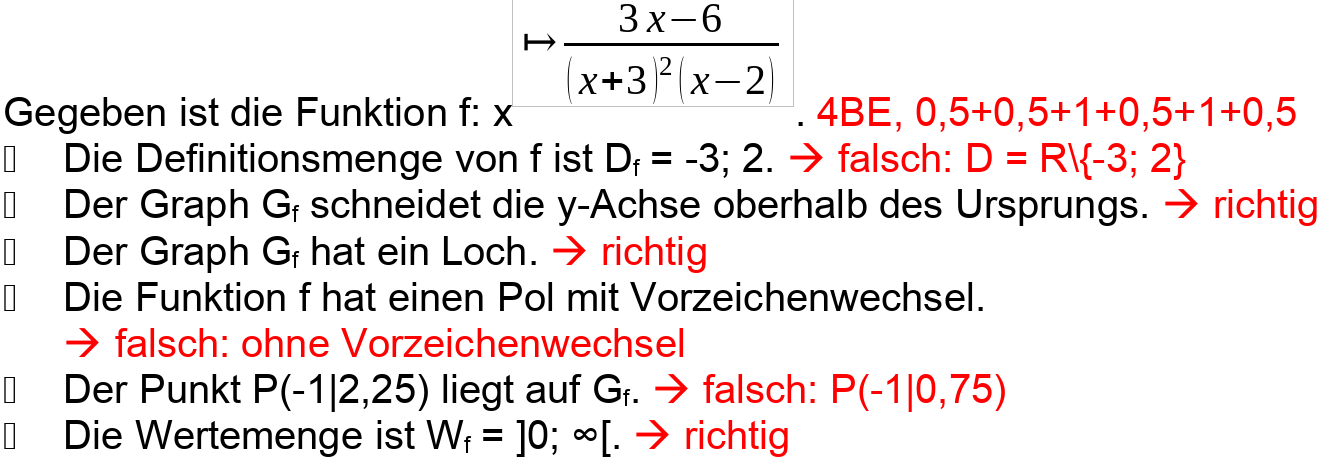
\includegraphics[width=\linewidth]{Q11_1KlausurJanuar2022_ml1.png}

\Aufgabe{2: Musterlösung}
\includegraphics[width=\linewidth]{Q11_2Klausur_4_loesungPyramide.png}


%%%%%%%%%%%%%%%%%%%%%%%%%%%%%%%%%%%%%%%%%%%%%%%%%%%%%%
%%%%%%%%%%%%%%%%%%%%%%%%%%%%%%%%%%%%%%%%%%%%%%%%%%%%%%
\end{document}
